\section{Vorstellung Projektergebnisse}\label{sec:projektergebnisse}
    Der gesamte Quellcode ist neben dem bereitgestelltem zip-Archiv auch auf GitHub unter \url{https://github.com/crochethk/mpa_project} abrufbar.

    Bei der Ausarbeitung wurde viel Wert darauf gelegt, den Quellcode bestmöglich mittels \emph{doc comment}s zu dokumentieren. Deshalb wird hier eher das grobe Zusammenspiel der Komponenten betrachtet und für evtl. Schnittestellendetails etc. auf den Quellcode\footnote{bzw. \ilc{rustdoc}, siehe \nameref{sec:extras}} verwiesen.

    \subsection{Bestandteile der Bibliothek}
        Die Bibliothek hat den Namen \ilc{mpa\_lib} und ist in folgende Module eingeteilt:

        \begin{itemize}
            \tightlist
            \item
            \ilc{mp\_int}: \textit{siehe unten}
            \item
            \ilc{utils}: Enthält mehr oder weniger lose Hilfsfunktionen und -strukturen, die von anderen Teilen der Bibliothek verwendet werden.
        \end{itemize}

        Des Weiteren sind eine CLI (\texttt{src/bin/demo\_cli.rs}) und mehrere Beispiele (\texttt{examples/*.rs}) vorhanden. Hierzu mehr in \autoref{sec:extras}.

    \subsubsection*{Modul \ilc{mp\_int}}
        Dieses Modul enthält den Datentyp und die Funktionalität für \mpi.

        \paragraph{\ilc{struct MPint}}
            Dieser Datentyp repräsentiert die \mpi\ und spielt dementsprechend die Hauptrolle in der Implementierung. Der Alias \ilc{DigitT} definiert dabei den Typ der Ziffern im internen Zahlensystem.

            \begin{figure}[H]
                \centering
                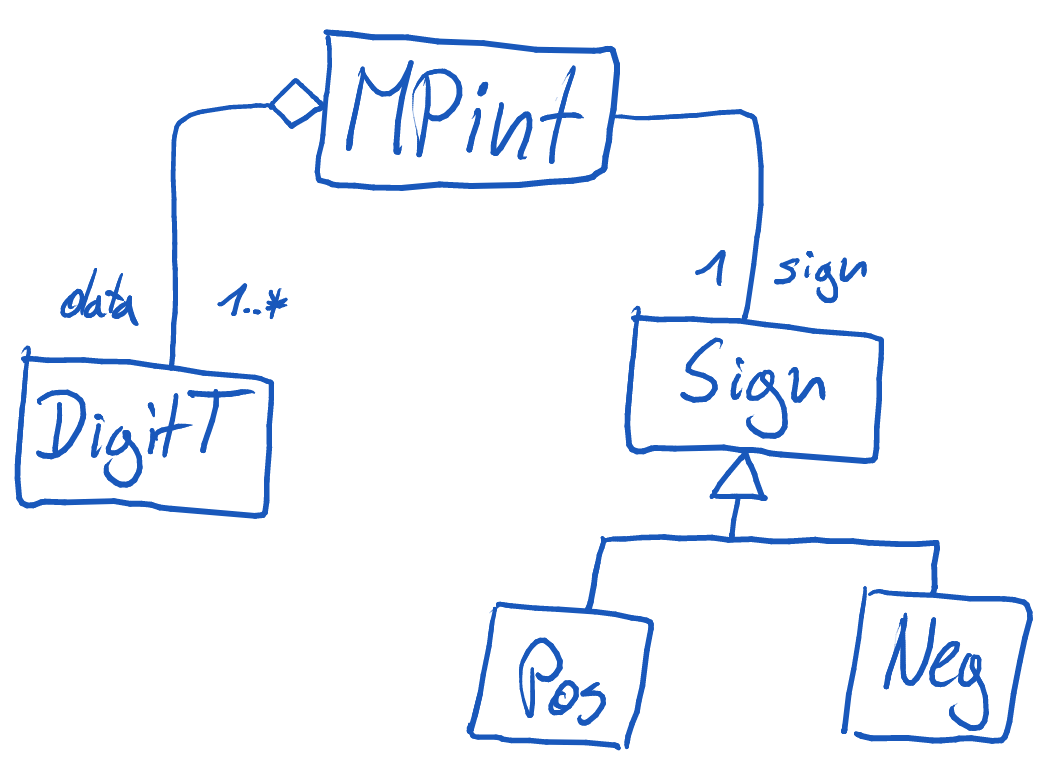
\includegraphics[width=0.5\linewidth]{images/cdmpint}
                \caption{Übersicht des \mpi\ Datentyps}
                \label{fig:cdmpint}
            \end{figure}

            Für \ilc{MPint} sind diverse \ilc{trait}s der Standardbibliothek implementiert.
            Insbesondere seien hier erwähnt:

            \begin{itemize} \tightlist
                \item die binären, arithmetischen Operatoren (\ilc{+}, \ilc{-}, \ilc{*}, \ilc{+=}),
                \item der unäre Negationsoperator (''\ilc{-x}'') und
                \item die binären Vergleichsoperatoren (\ilc{==}, \ilc{>}, \ilc{>=}, \dots)
            \end{itemize}

            Sie erlauben einen mit normalen Zahlen vergleichbaren Umgang mit den \mpi{}. Die arithmetischen Operatoren greifen dabei auf die in \autoref{sec:impldetails} angesprochenen Funktionen zurück.

            Es gibt diverse Möglichkeiten\footnote{Diese lassen sich hervorragend mit dem erwähnten Negationsoperator kombinieren, um negative \mpi\ zu erzeugen}, Instanzen zu erzeugen, u.a.:

            \begin{itemize}
                \item
                \ilc{MPint::new(u128)} \\
                    $\rightarrow$ aus nativen, vorzeichenlosen Integern
                \item
                \ilc{MPint::new(Vec<DigitT>)} bzw. Makro \ilc{mpint!(a\textsubscript{0}, a\textsubscript{1}, ...)} \\
                    $\rightarrow$ aus einer Liste an Ziffern
                \item
                \ilc{from\_hex\_str(\&str)} bzw. \ilc{from\_dec\_str(\&str)} \\
                    $\rightarrow$ aus Hex- bzw. Dezimal-Strings
            \end{itemize}

            Die \ilc{MPint::new(\dots)} Konstruktoren werden durch den benutzerdefinierten \ilc{trait}\\ \ilc{CreateNewFrom<T>} ermöglicht.

            Wie bereits erwähnt wird in Unit-Tests von Python Gebrauch gemacht. Das Vorgehen ist in zwei Phasen unterteilt:
            \begin{enumerate}
                \item Mit \ilc{mpint\_tests::verify\_arithmetic\_result(\dots)} wird die Operation und deren Ergebnis an eine Funktion in \ilc{mpint\_test\_helper.py} übergeben. Zurück kommt ein Tupel, mit der Information, ob das Ergebnis stimmt und einer passenden textuellen Meldung.

                \item Das Makro \ilc{mpint\_tests::create\_op\_correctness\_tester!} dient dazu, Code Duplikate zu vermeiden. Es erstellt für einen gegebenen Operator die entsprechend angepasste Test-Funktion. Hier ist der eigentliche \ilc{assert!} enthalten, welcher die vom Python-Skript erhaltenen Daten nutzt.
            \end{enumerate}


    \subsection{Bibliothek im eigenen Projekt nutzen} \label{sec:eigenesprojekt}
        Am Beispiel eines neuen Binary-Projekts wird jetzt gezeigt, wie sich die Bibliothek einbinden lässt.

        \paragraph*{Voraussetungen}
        Im Folgenden wird davon ausgegangen, dass Rust mit dem \href{https://rustup.rs}{\ilc{rustup}} Installer und der Standard-Toolchain eingerichtet wurde.

        \paragraph*{Schritte}

\begin{enumerate}
    \item Neues Binary-Projekt erstellen:

\begin{lstlisting}[language=bash]
cargo new my_new_project
\end{lstlisting}

    \item Library zum Projekt hinzufügen:
    \begin{itemize}
        \item \textit{Option 1} -- Direkt mit Git-Repository verknüpfen

\begin{lstlisting}[language=bash]
cd my_new_project
cargo add --git https://github.com/crochethk/mpa_project.git
\end{lstlisting}

        \item \textit{Option 2} -- Lokale Kopie nutzen
        \begin{itemize}
            \item Hole Library (z.B. Repo klonen)

\begin{lstlisting}[language=bash]
git clone https://github.com/crochethk/mpa_project.git
\end{lstlisting}

            \item Nach diesen Schritten ist die Ordnerstruktur in etwa: \\
                \begin{minipage}{10cm}
                \dirtree{%
                .1 /.
                .2 mpa\_project/.
                .2 my\_new\_project/.
                }
                \end{minipage}

            \item Verknüpfe mit lokaler Library

\begin{lstlisting}[language=bash]
cd my_new_project
cargo add --path ../mpa_project
\end{lstlisting}

        \end{itemize}
    \end{itemize}

    \item Library in \ilc{my\_new\_project} verwenden
    \begin{itemize}
        \item Inhalt von \ilc{my\_new\_project/src/main.rs} ersetzen

\begin{lstlisting}[language=Rust, style=boxed]
use mpa_lib::mp_int::*;

fn main() {
    println!("{}", mpint!(1,2));
}
\end{lstlisting}

        \item Ausführen\footnote{Ergebnis entspricht $1 \cdot (2^{64})^0 + 2 \cdot (2^{64})^1$}

\begin{lstlisting}[language=bash]
cargo run
# Out: 36893488147419103233
\end{lstlisting}


    \end{itemize}
\end{enumerate}

    \subsection{Unit-Tests ausführen}
     Aufgrund \ilc{pyo3} ist, zusätzlich zu den Voraussetzungen aus \autoref{sec:eigenesprojekt},  \href{https://pyo3.rs/main/getting-started}{mindestens eine \ilc{Python 3.7} Umgebung notwendig}.

    Um alle Tests auszuführen reicht folgender Befehl:
    \begin{lstlisting}[language=bash]
cargo test --all
    \end{lstlisting}
